% Copyright 2009--2014  Ed Bueler

%\documentclass[10pt,hyperref={pdfpagelabels=false}]{beamer}
\documentclass[10pt]{beamer}

\mode<presentation>
{
  \usetheme{Hannover}
  % or ...

  \usecolortheme{crane}

  \setbeamercovered{transparent}
  % or whatever (possibly just delete it)
  
  \setbeamerfont{frametitle}{size=\large}
}

\usepackage[english]{babel}
\usepackage[latin1]{inputenc}
\usepackage{times}
\usepackage[T1]{fontenc}
% Or whatever. Note that the encoding and the font should match. If T1
% does not look nice, try deleting the line with the fontenc.

\usepackage{empheq}
\usepackage{amsmath}
\usepackage{esint}
\usepackage{animate}
\usepackage{xspace}
\usepackage{verbatim}
\usepackage{hyperref}


\title{EXTRA SLIDES on Numerical modelling}

\author{Ed Bueler}

\institute{
Dept of Mathematics and Statistics \\
and Geophysical Institute \\
University of Alaska, Fairbanks}

\lecture[1]{Numerical modelling of ice sheets and ice shelves}{lecture-text}


\date{September 2014 \\ Karthaus Summer School}


% optional outline at start of each section
\AtBeginSection[]
{
  \begin{frame}<beamer>
    \frametitle{Outline}
    \tableofcontents[currentsection,hideallsubsections]
  \end{frame}
}


% If you wish to uncover everything in a step-wise fashion, uncomment:
%\beamerdefaultoverlayspecification{<+->}

\newcommand{\bg}{\mathbf{g}}
\newcommand{\bq}{\mathbf{q}}
\newcommand{\bu}{\mathbf{u}}
\newcommand{\bw}{\mathbf{w}}

\newcommand{\bA}{\mathbf{A}}
\newcommand{\bbF}{\mathbf{F}}
\newcommand{\bU}{\mathbf{U}}

\newcommand{\ddt}[1]{\ensuremath{\frac{\partial #1}{\partial t}}}
\newcommand{\ddx}[1]{\ensuremath{\frac{\partial #1}{\partial x}}}
\newcommand{\ddy}[1]{\ensuremath{\frac{\partial #1}{\partial y}}}
\newcommand{\pp}[2]{\ensuremath{\frac{\partial #1}{\partial #2}}}
\renewcommand{\t}[1]{\texttt{#1}}
\newcommand{\eps}{\epsilon}
\newcommand{\grad}{\nabla}
\newcommand{\Div}{\nabla\cdot}
\newcommand{\strainrate}{D}
\newcommand{\devstress}{\tau}

\newcommand{\Matlab}{\textsc{Matlab}\xspace}
\newcommand{\Octave}{\textsc{Octave}\xspace}

\newcommand{\exer}[2]{\medskip\noindent \textbf{#1.}\quad #2}
\mode<presentation>{
\newcommand{\slidepage}[1]{slide \pageref{#1}}
}

\newcommand{\mname}[1]{\href{http://www.dms.uaf.edu/~bueler/karthaus/mfiles/#1}{\texttt{#1}}}

\newcommand{\txtinput}[1]{ \scriptsize \verbatiminput{#1} } %a

\newcommand{\txtinputtiny}[1]{ \tiny \verbatiminput{#1} } %a

%\newcommand{\mmessage}[1]{\begin{center}
%\emph{see code} \url{http://www.dms.uaf.edu/~bueler/karthaus/mfiles/#1.m}
%\end{center}}
\newcommand{\mmessage}[1]{\begin{center}
\emph{see code} \texttt{#1.m}
\end{center}}

%\newcommand{\mmess}[1]{\vspace{-0.1in}\begin{center}
%\fbox{\url{http://www.dms.uaf.edu/~bueler/karthaus/mfiles/#1.m}}
%\end{center}}
\newcommand{\mmess}[1]{\vspace{-0.1in}\begin{center}
\fbox{\texttt{#1.m}}
\end{center}}

\newcommand{\minput}[1]{
\scriptsize \verbatiminput{mfiles/#1.slim.m} %a
\vspace{-2mm}
\scriptsize \mmess{#1}
\normalsize
}

\newcommand{\minputtiny}[1]{
\tiny \verbatiminput{mfiles/#1.slim.m} %a
\vspace{-4mm}
\scriptsize \mmess{#1}
\normalsize
}


\begin{document}

\graphicspath{{../photos/}{../pdffigs/}}

\begin{frame}
  \maketitle
\end{frame}

% Copyright 2009--2014  Ed Bueler

\section{technical skills}

\begin{frame}[fragile]
\frametitle{technical skills}

\begin{itemize}
\item next two slides are free advice on technical skills needed for numerical ice sheet modelling
  \begin{itemize}\small
  \item[$\circ$] you get what you pay for
  \normalsize
  \end{itemize}
\end{itemize}
\end{frame}


\begin{frame}
\frametitle{technical skills for numerical ice sheet modelling }

\begin{itemize}
\item you need comfort in a technical computing environment, including
  \begin{itemize}\small
  \item[$\circ$] an editor,
  \item[$\circ$] a scripting/prototyping language (Matlab, Python, etc.),
  \item[$\circ$] a compiled language (C or Fortran),
  \item[$\circ$] a version control system (Subversion, git, etc.), and
  \item[$\circ$] some tools for NetCDF files
  \normalsize
  \end{itemize}
\item you need willingness to read physics, numerical analysis, computer science, etc.~books
\end{itemize}
\end{frame}


\begin{frame}
\frametitle{technical skills for numerical ice sheet modelling 2}

\begin{itemize}
\item you should \emph{never} re-invent the wheel for basic numerics like these, \emph{except} to write throw-away codes to help you understand them:
  \begin{itemize}
  \item[$\circ$] numerical linear algebra
  \item[$\circ$] mesh generation
  \item[$\circ$] finite element assembly and solve
  \end{itemize}
\item try existing open source ice flow models:
  \begin{itemize}
  \item[$\circ$] shallow comprehensive models:
    \begin{itemize}
    \item GLIMMER
    \item SICOPOLIS
    \item PISM
    \end{itemize}
  \item[$\circ$] open source higher-order/Stokes models:
    \begin{itemize}
    \item Elmer/Ice
    \item ISSM
    \end{itemize}
  \end{itemize}
\end{itemize}
\end{frame}

% Copyright 2009--2012  Ed Bueler

\begin{frame}{\textsl{POSTSCRIPT}  have I oversold diffusivity?} 

\begin{itemize}
\item I have asserted that the default model for ice sheets, the SIA, is a \emph{diffusion} like the heat equation
\item recall the analogy:

\bigskip
\begin{tabular}{ccc}
\emph{heat eqn} & $\leftrightarrow$ & \emph{SIA} \\ \hline
$T_t = \Div\left(D \grad T\right)$ & $\leftrightarrow$ & $H_t = M + \Div\left(D \grad h\right)$ \\
$D=D(x,y)$ & $\leftrightarrow$ & $D = \Gamma H^{n+2} |\grad h|^{n-1}$ \\
\end{tabular}

\bigskip
\item have I oversold this diffusivity analogy?
  \begin{itemize}
  \item[$\circ$] possibly
  \item[$\circ$] I've acknowledged there are ``issues''
  \end{itemize}
\item but it turns out there is some robustness to the analogy
\end{itemize}
\end{frame}


\begin{frame}{have I oversold diffusivity? 2}

\emph{DIFFUSIVE IDEA 1}: rough beds have the effect of \emph{reducing} diffusivity
\begin{itemize}
\item define the local bed topography by removing the local mean over some range $\lambda \approx 10$ km:
\small
   $$\tilde b(x,\xi) = b(x+\xi) - \fint_{-\lambda}^\lambda b(x+\xi)\,d\xi$$
\normalsize
\item define this average of the local bed:
\small
	$$\theta(x) = \left(\fint_{-\lambda}^\lambda \left(1 - \frac{\tilde b(x,\xi)}{H(x)}
                           \right)^{-(n+2)/n}\,d\xi\right)^{-1/n}$$
\normalsize
\item using a multiple-scales analysis, Schoof [2003] says you will get closer to solving the Stokes equations by making these two modifications of the SIA:
  \begin{itemize}
  \item[$\circ$] smooth the bed
  \item[$\circ$] but don't lose track of the smoothed-away local bed roughness; use it to reduce the diffusivity:
  \small
  		$$D_{\text{new}} = \theta D \qquad \text{where } 0 \le \theta \le 1$$
  \end{itemize}
\end{itemize}
\end{frame}


\begin{frame}{have I oversold diffusivity? 3}

\emph{DIFFUSIVE IDEA 2}: the large-scale effect of \emph{sliding} in ice streams (\emph{addressed in next section}), is also diffusive
\begin{itemize}
\item suppose that, for an ice stream modeled by the SSA equation
   $$\left(2 A^{-1/n} H |u_x|^{1/n - 1} u_x \right)_x - C|u|^{m-1}u = \rho g H h_x$$
we assume that the basal resistance term balances the driving stress:
   $$- C|u|^{m-1}u = \rho g H h_x$$
\item then the ice stream geometry evolves by a non-SIA diffusion,
	$$H_t = M + \Div\left(D\,\grad h\right) \qquad \text{where } D = C' H^{(1/m)+1}|\grad h|^{(1/m)-1}$$
\item this ``outer problem'' is part of a matched asymptotic expansion that \emph{does a good job of tracking the grounding line in a marine ice sheet} [Schoof, 2007]
\end{itemize}
\end{frame}


% Copyright 2009--2012  Ed Bueler

%\section{free boundary problems}

\begin{frame}{\emph{POSTSCRIPT} on free boundary value problems}

\begin{itemize}
\item ice sheet/shelf modelling means free boundary problems
\item Hutter [1999] identifies some:
\end{itemize}
\begin{center}
  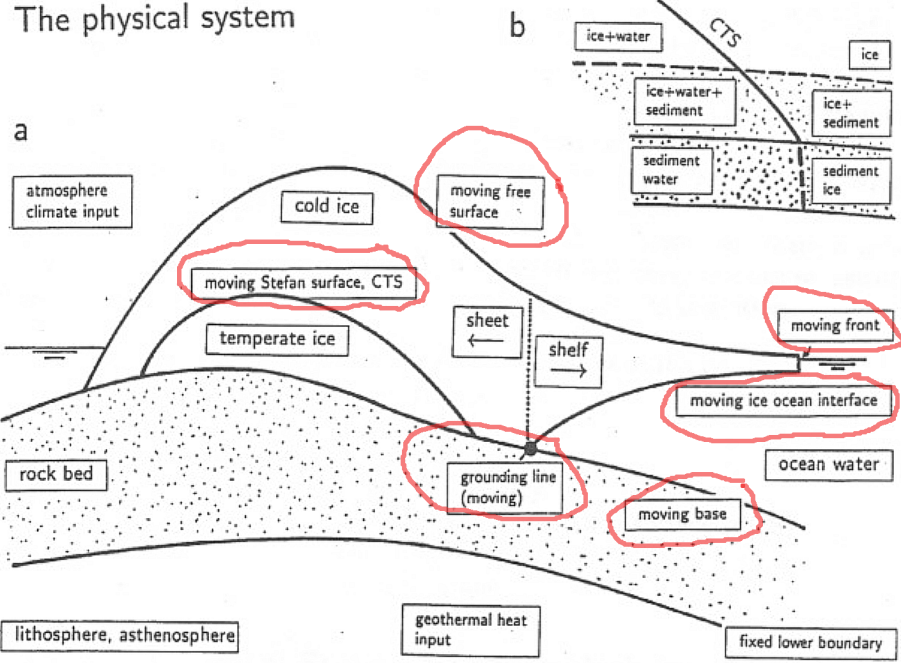
\includegraphics[width=0.8\textwidth]{photos/freehutter}
\end{center}
\end{frame}


\begin{frame}{what is a ``free boundary''?}

\begin{itemize}
\item a \emph{free boundary} for a PDE is an unknown location at which there is a boundary condition
  \begin{itemize}
  \item[$\circ$] the location of the free boundary must be found at the same time as one solves the PDE problem
  \item[$\circ$] there must be enough additional information at a free boundary to determine its location
  \item[$\circ$] all free boundary problems are nonlinear, even if the PDE is linear
  \end{itemize}
\item classic \emph{example}:  consider an elastic membrane attached to a wire frame and stretched over an obstacle:
\end{itemize}

\begin{columns}
\begin{column}{0.5\textwidth}
\small
constraint:
  $$u \ge \psi$$

in locations where $u>\psi$, solve:
  $$\grad^2 u = 0$$
  
\emph{where is the free boundary, and what facts about $u$ are true there?}
\end{column}
\begin{column}{0.5\textwidth}
  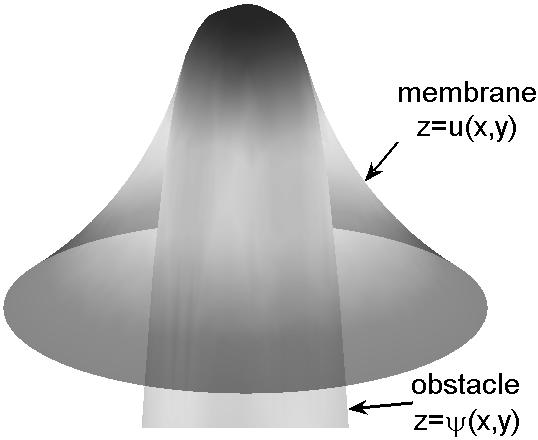
\includegraphics[width=1.0\textwidth]{photos/classicalobs}
\end{column}
\end{columns}
\end{frame}


\begin{frame}{free boundary value problem 1: polythermal ice}

\small
\begin{itemize}
\item by volume, majority of ice sheet is \emph{cold} ($T < 0\phantom{|}^\circ\text{C}$)
\item \dots but there is some ice which is \emph{temperate}, where $T = 0\phantom{|}^\circ\text{C}$ \emph{and} there is a positive liquid fraction within the ice matrix
\item ice sheets are \emph{polythermal}
\item boundary between cold and temperate ice is ``CTS'' (= cold-temperate transition surface):
  \begin{itemize}
  \item[$\circ$] must be found, as free boundary, when solving conservation of energy equation (``Stefan problem'')
  \item[$\circ$] can be tracked explicitly [Greve, 1997]
  \item[$\circ$] or treated as a level surface of the enthalpy variable [Aschwanden et al, 2012]
  \end{itemize}
\end{itemize}

\begin{center}
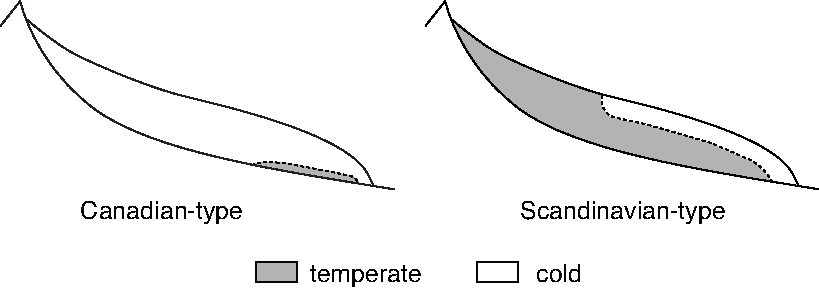
\includegraphics[width=0.8\textwidth]{photos/polythermal_types}
\end{center}
\end{frame}


\begin{frame}{free boundary value problem 2: for ice streaming}

%\vspace{-0.2in}
\begin{itemize}
\item  Schoof's [2006] insight, for diagnostic case
  $$\text{SSA + (plastic till)} = \begin{pmatrix}
\text{well-posed free boundary problem} \\ \text{for location \emph{and} velocity of sliding}
\end{pmatrix} $$
\item ``plastic till'' means the basal strength (resistance) is given by a yield stress $\tau_c$:  \qquad $\vec\tau_b = \tau_c \mathbf{v}_b / |\mathbf{v}_b|$
\item Schoof's scheme is a \emph{whole ice sheet form} of MacAyeal's [1989] individual ice stream model
\end{itemize}

\begin{columns}
\begin{column}{0.5\textwidth}
\begin{center}
  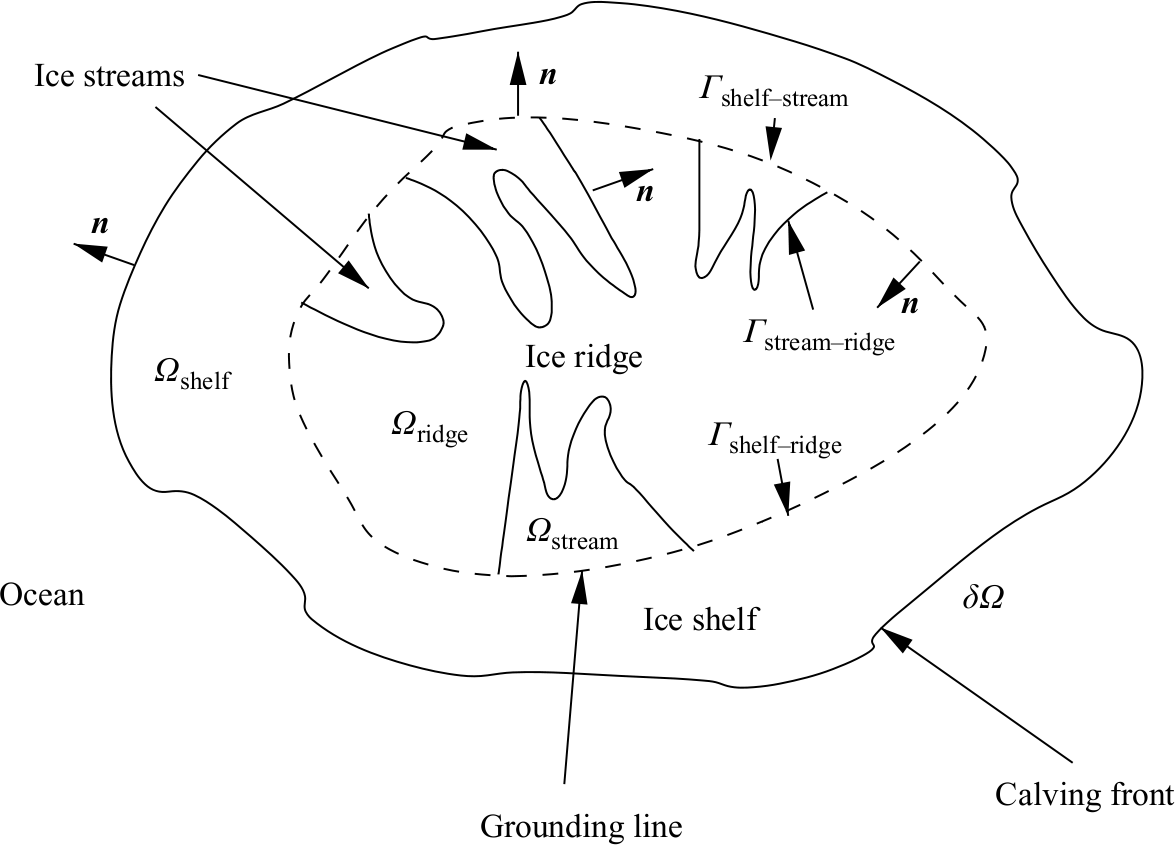
\includegraphics[width=1.0\textwidth]{photos/schoof_planform}
\end{center}
\end{column}
\begin{column}{0.5\textwidth}
\begin{center}
  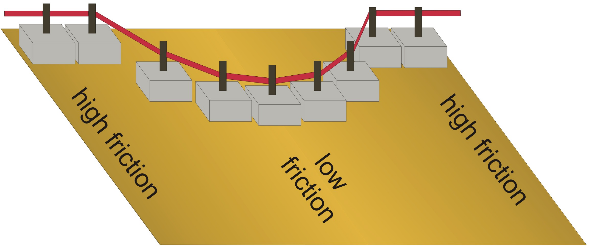
\includegraphics[width=0.95\textwidth]{photos/schoof_sliders}
\end{center}
\end{column}
\end{columns}
\end{frame}


\begin{frame}{free boundary problem 3: for grounded ice sheet margin}

\begin{itemize}
\item side-by-side comparison, \emph{classical elastic membrane problem} versus \emph{steady ice sheet problem}
\end{itemize}
\small
\begin{columns}[T]
\begin{column}{0.4\textwidth}
constraint:
  $$u \ge \psi$$

where $u>\psi$, solve:
  $$\grad^2 u = 0$$

\bigskip
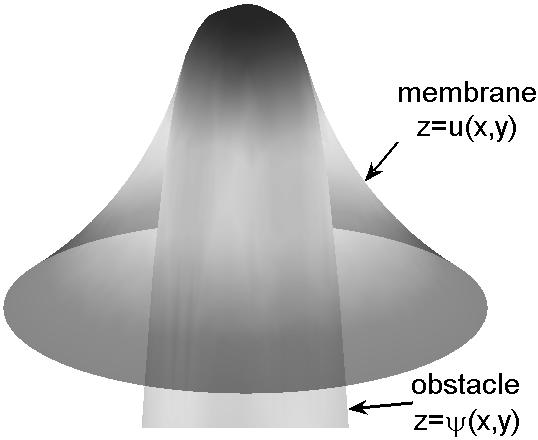
\includegraphics[width=0.8\textwidth]{photos/classicalobs}
\end{column}
\begin{column}{0.6\textwidth}
constraint:
  $$h \ge b \qquad \iff \qquad H \ge 0$$

where $h>b$, solve steady SIA:
  $$0 = M + \Div \left(\Gamma H^{n+2} |\grad h|^{n-1} \grad h \right)$$

\bigskip
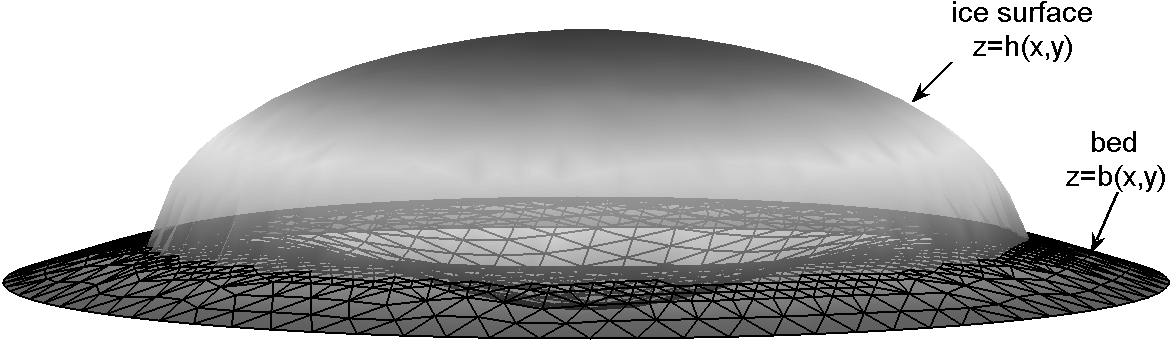
\includegraphics[width=0.9\textwidth]{photos/capnonflatobs}
\end{column}
\end{columns}
\end{frame}


\begin{frame}{free boundary problems: why do they matter?}
\begin{itemize}
\item the location of the free boundary may \emph{be} the glaciological question
\item free boundaries are always locations of \emph{loss of smoothness} relative to fixed boundary solutions
     \begin{itemize}
     \item[$\circ$] numerical error may be dominated by errors near these free boundaries, 
     \item[$\circ$] hard to know whether model results at free boundaries are poor because of numerical problems or because of missing physical processes
     \end{itemize}
\end{itemize}
\end{frame}




\end{document}

